\section{بخش سوم: حذف پس‌زمینه و استخراج متن}

\begin{stepbox}
\field{هدف این بخش (بخش ۳)}{
کم کردن تصویر اصلی از تصاویر تولید شده در مرحله‌ی قبل (نقشه‌ی تخمینیِ پس‌زمینه) به منظور حذف اثر سایه، و سپس یافتن یک سطح آستانه‌ی مناسب برای جداسازی نهاییِ متن از پیش‌زمینه.
}
\end{stepbox}

\subsection{کد پیاده‌سازی و منطق آن}
برای این عملیات، تفریق ساده‌ی ریاضی در پایتون می‌تواند منجر به خطای سرریزِ منفی (\lr{Underflow}) در متغیرهای ۸ بیتی شود. به همین دلیل از تابع امنِ کتابخانه‌ی \lr{OpenCV} استفاده کردیم:

\begin{codebox}[\lr{Subtraction and Thresholding}]
\begin{lstlisting}[language=Python]
# Subtract original image from background map (avoids negative values)
diff_img = cv2.subtract(dilated, img)

# Apply optimal threshold (T=40)
ret, thresh_img = cv2.threshold(diff_img, 40, 255, cv2.THRESH_BINARY)

# Invert colors (black text on white background)
final_result = cv2.bitwise_not(thresh_img)
\end{lstlisting}
\end{codebox}

\textbf{توضیح کد:}
تابع \lr{\texttt{cv2.subtract}} بسیار هوشمندانه عمل می‌کند؛ در محاسبات نوع \lr{\texttt{uint8}}، اگر حاصل تفریق منفی شود، این تابع مقدار را دقیقاً روی صفر (سیاه مطلق) قفل می‌کند. پس از تفریق، از آنجایی که مشکل روشناییِ متغیر حل شده، با یک تابع \lr{\texttt{cv2.threshold}} ساده مقادیر بالاتر از ۴۰ (که حالا همان پیکسل‌های متن هستند) را استخراج کردیم. در نهایت با \lr{\texttt{cv2.bitwise\_not}} خروجی را به فرم استانداردِ متون چاپی (متن سیاه روی کاغذ سفید) برگرداندیم.

\subsection{خروجی‌های تصویری و تحلیل دقیق آن‌ها}
در این بخش، ابتدا تصاویر تفاضل (\lr{Difference}) و سپس تصاویر خروجی نهاییِ آستانه‌گذاری شده را بررسی کردیم.

\begin{figure}[h!]
    \centering
    \begin{subfigure}{0.31\textwidth}
        \centering
        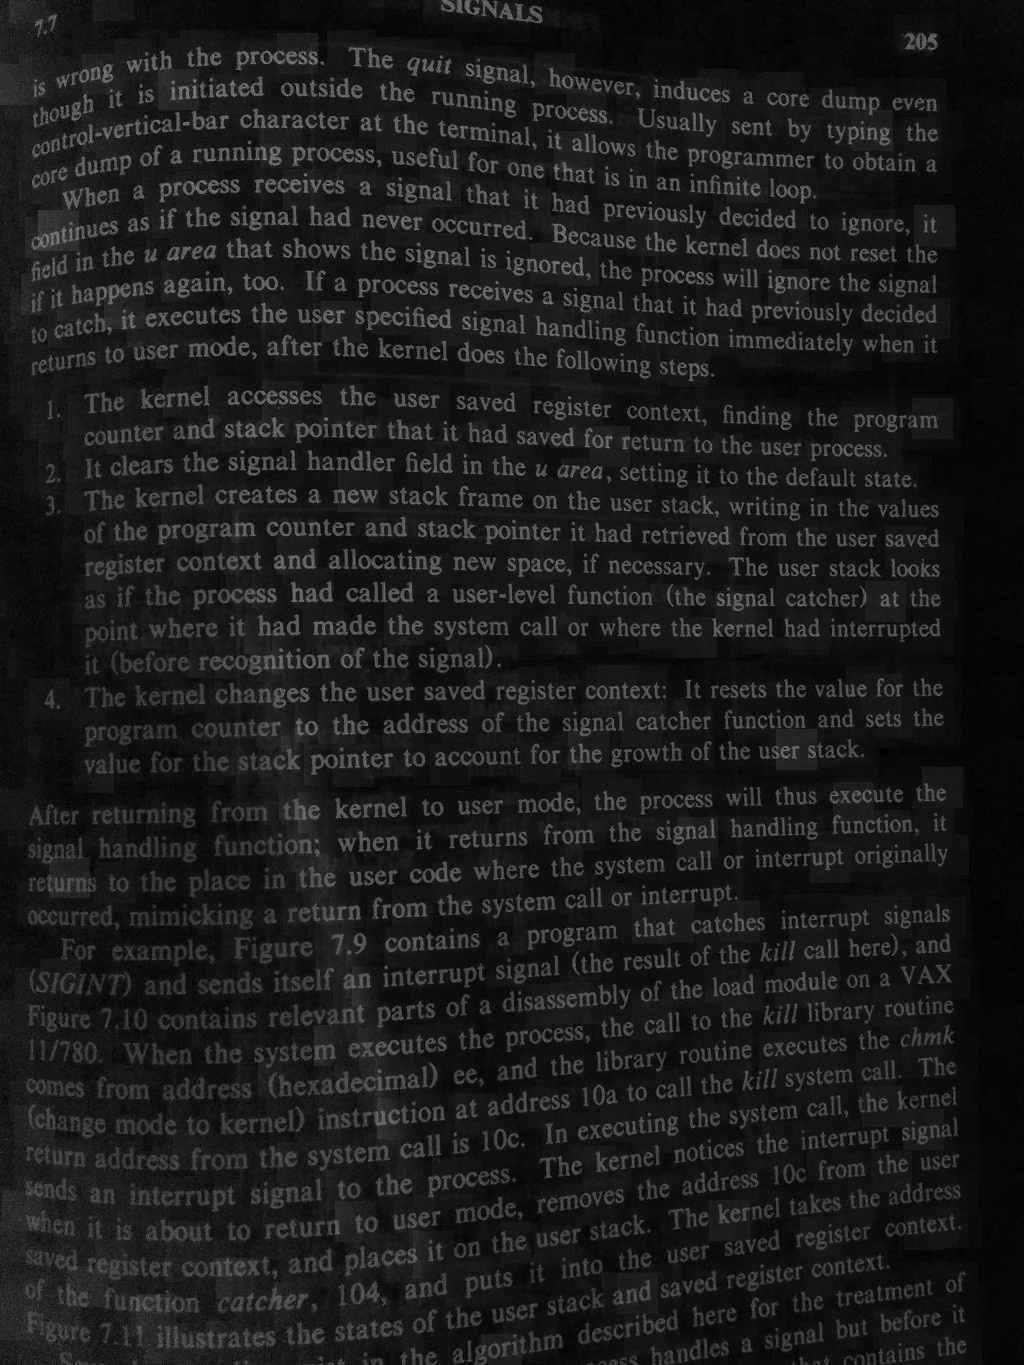
\includegraphics[width=\linewidth]{images/diff_41x41.jpg}
        \caption{تفاضل (پنجره ۴۱)}
    \end{subfigure}
    \hfill
    \begin{subfigure}{0.31\textwidth}
        \centering
        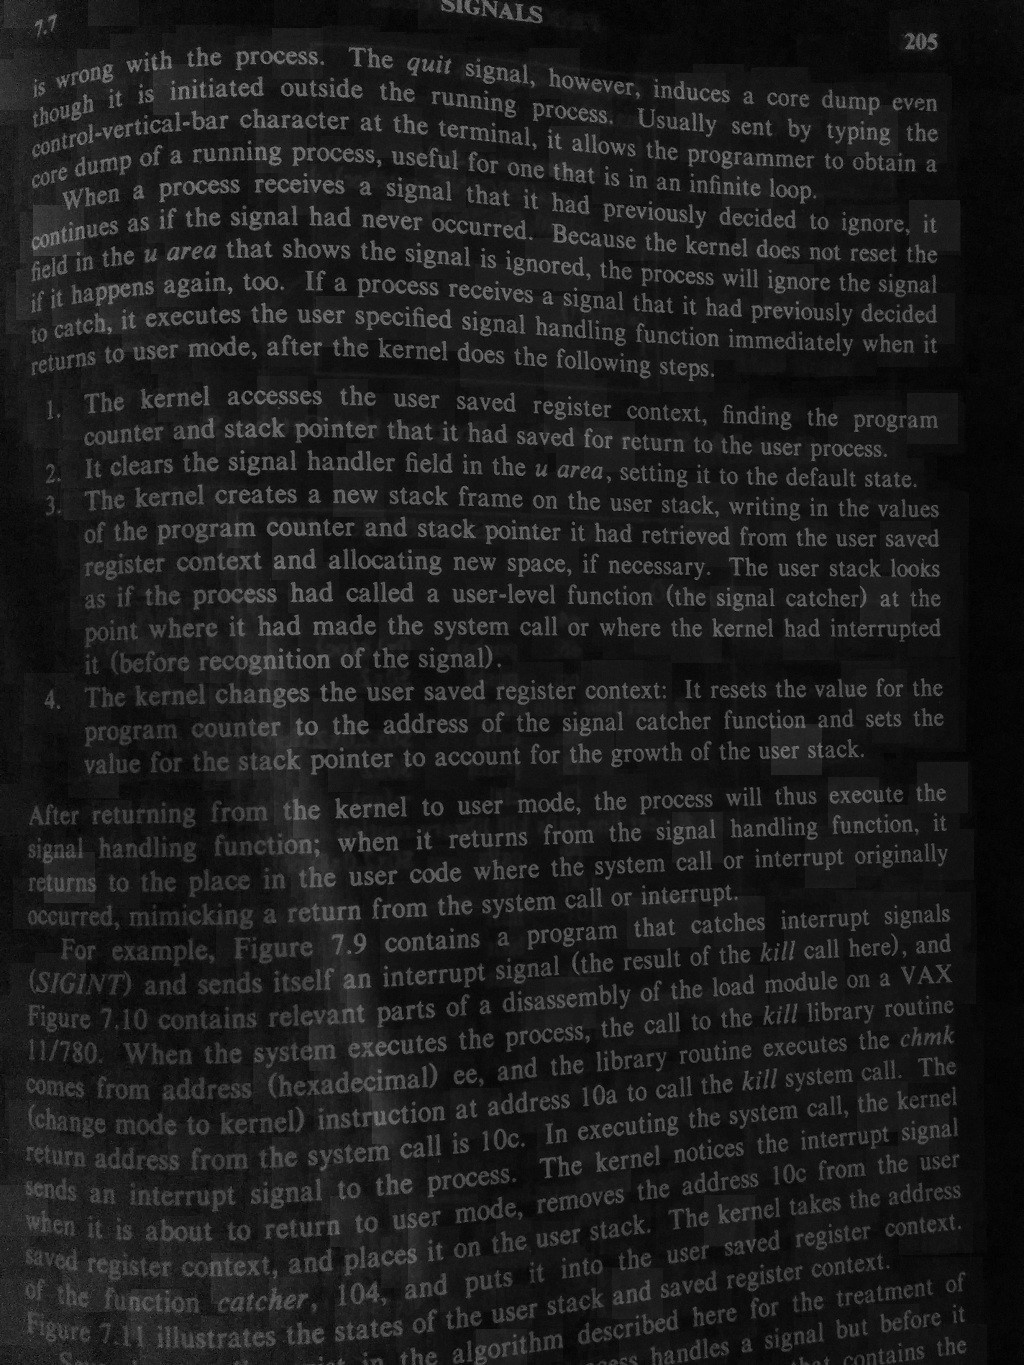
\includegraphics[width=\linewidth]{images/diff_51x51.jpg}
        \caption{تفاضل (پنجره ۵۱)}
    \end{subfigure}
    \hfill
    \begin{subfigure}{0.31\textwidth}
        \centering
        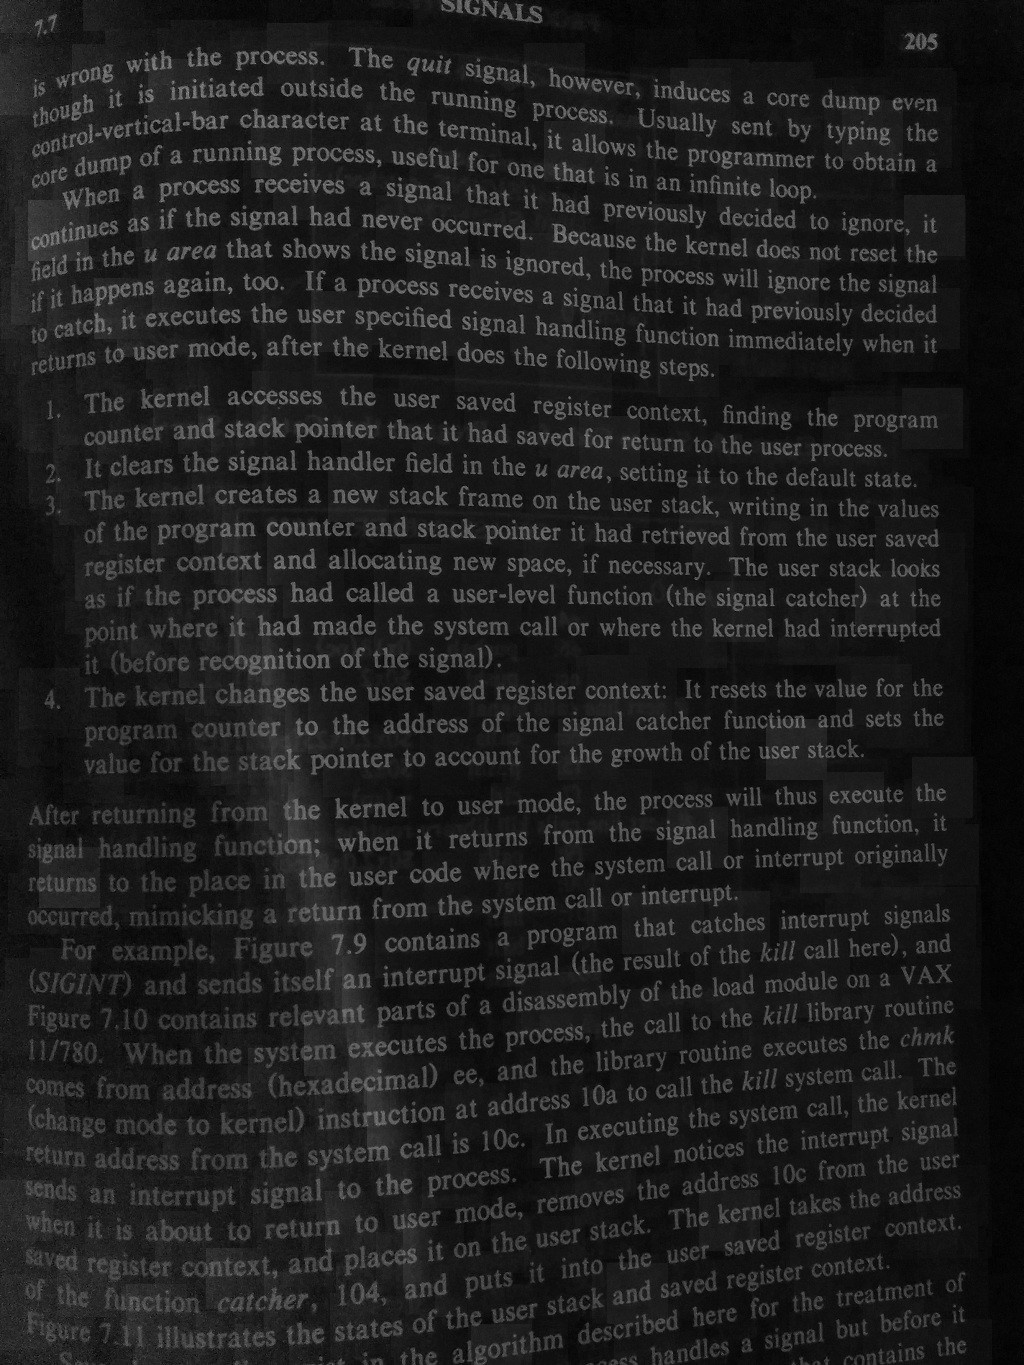
\includegraphics[width=\linewidth]{images/diff_61x61.jpg}
        \caption{تفاضل (پنجره ۶۱)}
    \end{subfigure}
    
    \vspace{0.4cm}
    
    \begin{subfigure}{0.31\textwidth}
        \centering
        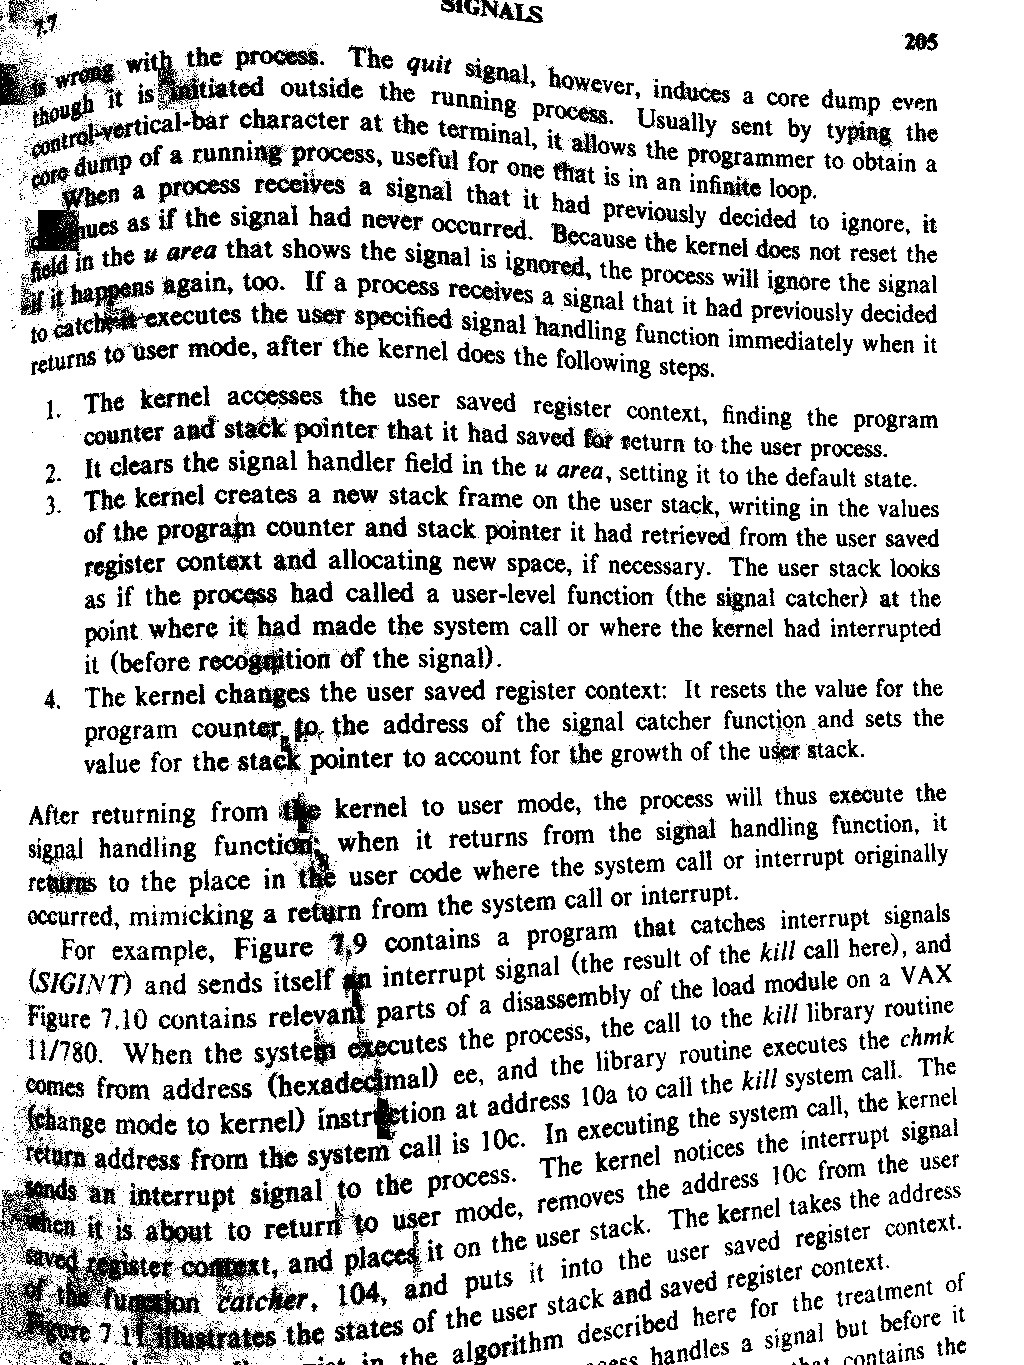
\includegraphics[width=\linewidth]{images/final_thresh_41x41.jpg}
        \caption{نهایی (پنجره ۴۱)}
    \end{subfigure}
    \hfill
    \begin{subfigure}{0.31\textwidth}
        \centering
        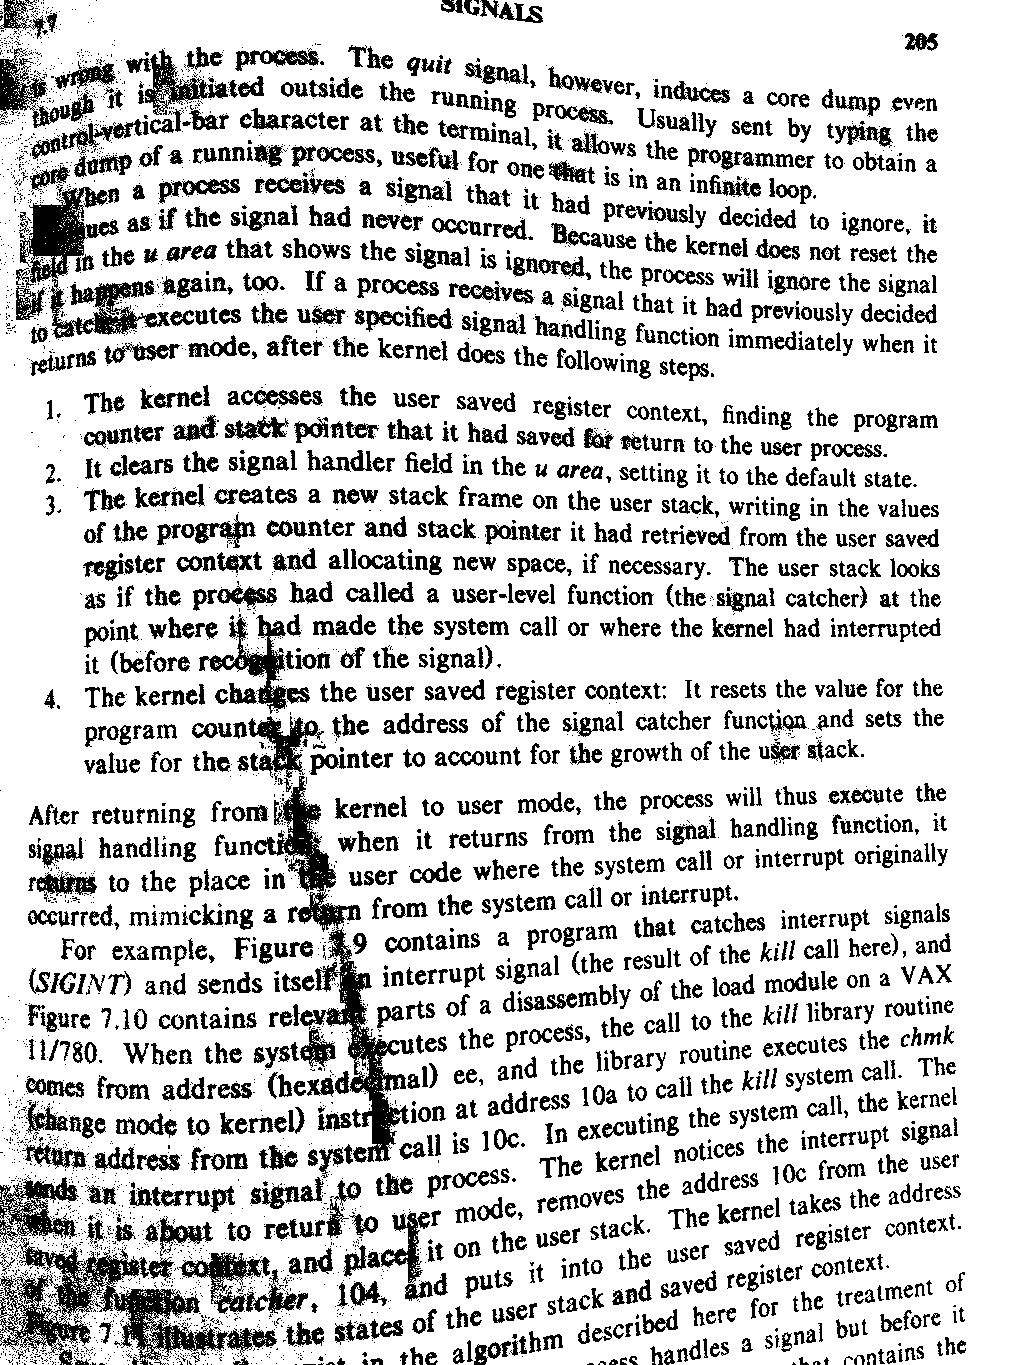
\includegraphics[width=\linewidth]{images/final_thresh_51x51.jpg}
        \caption{نهایی (پنجره ۵۱)}
    \end{subfigure}
    \hfill
    \begin{subfigure}{0.31\textwidth}
        \centering
        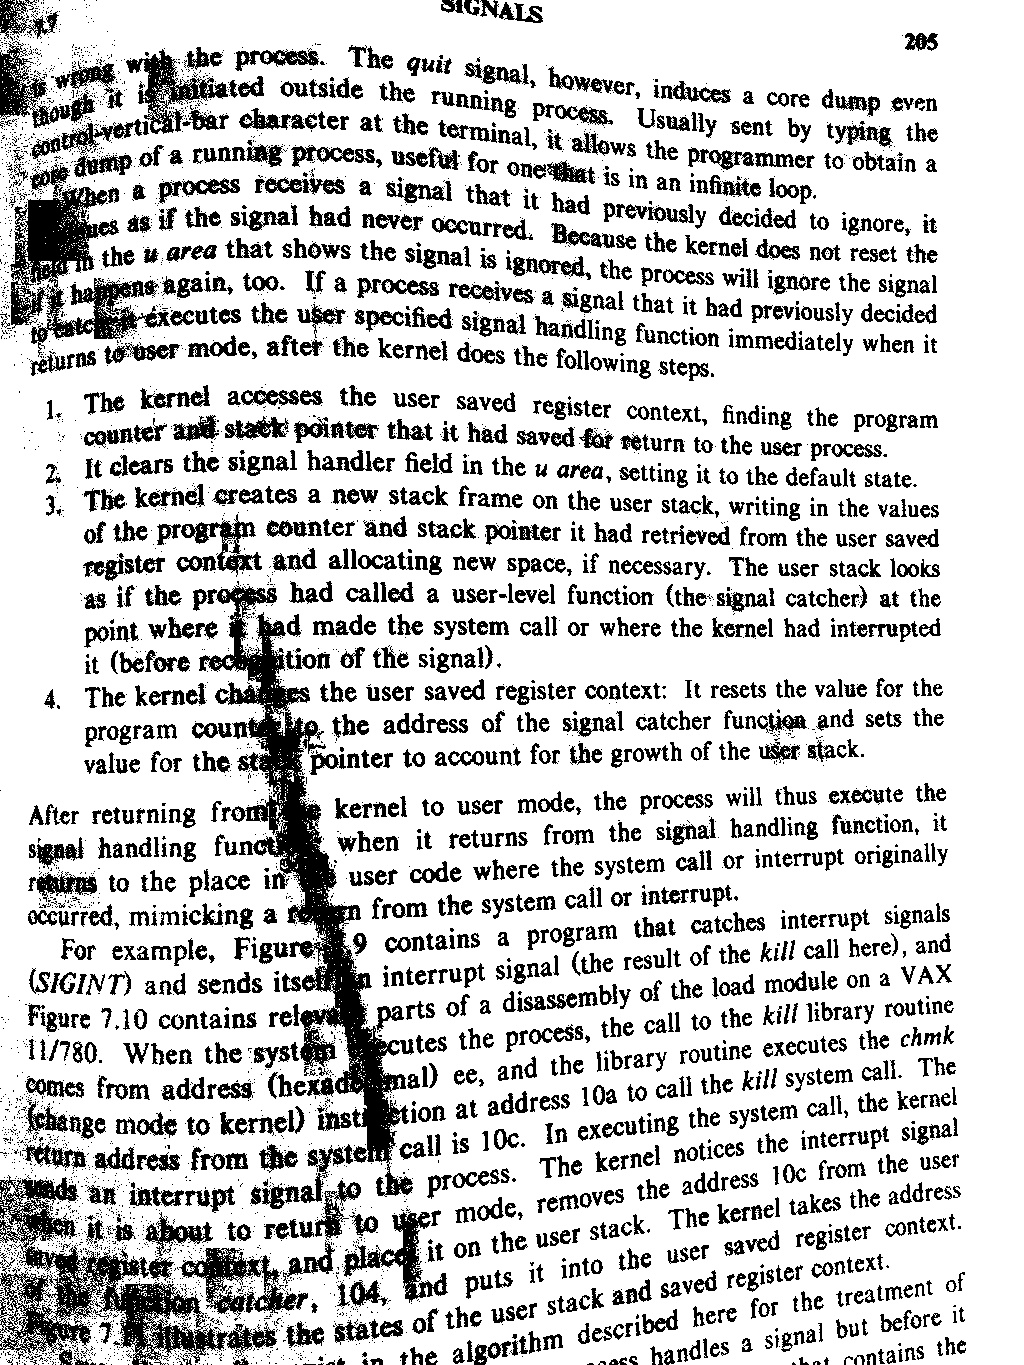
\includegraphics[width=\linewidth]{images/final_thresh_61x61.jpg}
        \caption{نهایی (پنجره ۶۱)}
    \end{subfigure}
    \caption{تصاویر تفاضل و نتیجه‌ی استخراج متن پس از حذف سایه}
    \label{fig:part3_diff_thresh}
\end{figure}

\textbf{کالبدشکافی عملیات تفریق و مقایسه‌ی پنجره‌ها:}
عمل تفریق به این شکل عمل می‌کند که در نواحیِ مربوط به کاغذ (چه زیر سایه، چه در روشنایی)، مقدار پیکسل در تصویر اصلی و تصویرِ \lr{Dilation} تقریباً برابر است؛ در نتیجه حاصل تفریق صفر (سیاه) می‌شود. اما در نواحیِ متن، چون تصویر اصلی تیره و نقشه \lr{Dilation} به رنگ روشنِ کاغذ درآمده، حاصل تفریق یک عدد مثبتِ بزرگ می‌شود. به همین دلیل در تصاویر تفاضل، متن‌ها مثل چراغ‌های درخشان روی پس‌زمینه‌ای تاریک پدیدار می‌شوند.
\begin{itemize}
    \item \textbf{برتری پنجره‌ی $41\times41$ در حفظ مرزها:} با بررسی دقیقِ لبه‌های سایه، متوجه می‌شویم که پنجره‌ی $61\times61$ به دلیل شعاعِ بزرگش، دچار پدیده‌ی «اثر حاشیه‌ای» (\lr{Edge Artifact}) شده است. یعنی این پنجره روشناییِ بخش‌های بیرون از سایه را به اشتباه به داخلِ مرزِ تاریکِ سایه نشت داده است. این امر باعث شد در تصویرِ نهاییِ آن، در لبه‌های سایه لکه‌های ضخیمِ سیاهِ خطا تولید شود. اما پنجره‌ی $41\times41$ به دلیل وسعتِ کمتر، هندسه‌ی واقعی سایه را بسیار دقیق‌تر حفظ کرد و خروجیِ نهاییِ تمیزتر و بهتری ارائه داد.
\end{itemize}
\newpage
\subsection{پاسخ به سوالات تمرین}
\textbf{نحوه پیدا کردن و مقدار سطح آستانه را مکتوب کنید.} \\
با تفریق تصویر اصلی از تصویر بسط‌یافته، اثر تغییرات تدریجیِ روشنایی (سایه مزاحم) به طور کامل خنثی گردید. در تصویرِ تفاضل، پس‌زمینه به مقداری نزدیک به صفر (سیاه) رسید و پیکسل‌های متن دارای مقادیر بزرگتر (روشن) شدند. با بررسی چشمیِ تصویرِ تفاضل و هیستوگرام آن به صورت تجربی، مقدار آستانه \lr{T = 40} انتخاب شد. این مقدار به اندازه‌ای بزرگ است که نویزهای جزئیِ پس‌زمینه را نادیده بگیرد، و به اندازه‌ای کوچک است که تمام پیکسل‌های مربوط به کاراکترهای متنی را حفظ کرده و به سفید کامل نگاشت کند.